\subsection{Implementação de WebServices no GSAN}

A estratégia de desenvolver o WebService internamente ao sistema GSAN, foi adotada, visando a possibilidade de reaproveitamento de toda regra de negócio, entidade, controlados dentre os demais artefatos que fazem parte do sistema.  Os novos serviços foram desenvolvidos sob tecnologias compatíveis com as utilizadas no sistema GSAN, utilizando a especificação JAX-WS (\textit{Java API for XML-BasedWeb Services}) para serem consumidos por sistemas externos através de submissões de arquivos do tipo XML, definidas no padrão de comunicação SOAP. Para tratar de conversões de arquivos XML para objetos e vice-versa está sendo utilizada a especificação do padrão JAXB (\textit{Java Architecture for XML Binding}), dessa forma estes serviços serão executados no mesmo servidor de aplicação.
Na prática será necessário importar ao projeto as seguintes bibliotecas descritas abaixo;

% LIBS UTILIZADAS
\begin{description}
	\item Prover suporte a configuração do End-Points (Serviços);
	\begin{itemize}
		\item jaxws-api-2.2.jar
		\item jaxws-rt.jar
		\item jaxws-tools.jar		
	\end{itemize}
	\item Fornecer suporte ao tratamento de serialização dos XML;
	\begin{itemize}
		\item jaxb-impl.jar
		\item jaxb-xjc.jar
		\item policy.jar
		\item stax-ex.jar
		\item stax2-api.jar
		\item streambuffer.jar
		\item woodstox-core-asl.jar		
	\end{itemize}
\end{description}

Após realizar a configuração das bibliotecas necessárias para implementação, foram definidos os seguintes novos serviços para atender as necessidades do \textit{Call Center} (figura 10):

\begin{figure}[!htb]
	\centering
	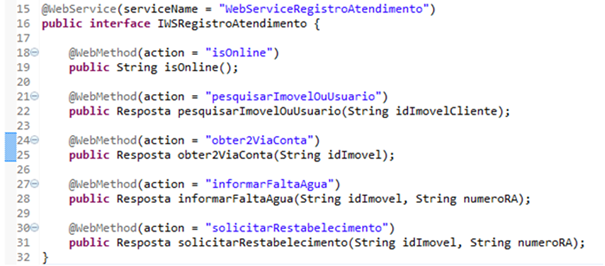
\includegraphics{figuras/implementacao_servicos.png}
	\caption{Interface dos serviços automatizados.}	
	Fonte - Autoria Própria
\end{figure}


Para definir a URL (\textit{Uniform Resource Locator}) de acesso ao \textit{WebService} será preciso atualizar o arquivo web.xml, declarando a servlet padrão definida na especificação do JAX-WS para esse propósito, conforme a figura 11:

\begin{figure}[!htb]
	\centering
	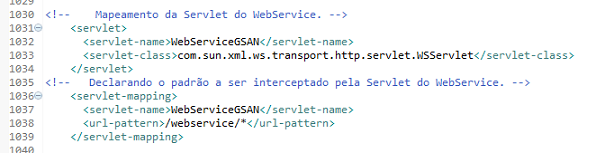
\includegraphics{figuras/declarando_servlet.png}
	\caption{Declaração da servlet do WebService.}	
	Fonte - Autoria Própria
\end{figure}


Feito isso, será preciso disponibilizar os novos serviços, definindo a classe concreta de implementação e o padrão de acesso que será adotado para a interface criada, para que as solicitações sejam interceptadas adequadamente redirecionadas ao \textit{EndPoints} corretos, com isso será necessário criar o arquivo com a seguinte nomenclatura \textit{sun-jaxws.xml}, localizado dentro do diretório WEB\_INF da aplicação, segue abaixo o conteúdo do arquivo, conforme a figura 12:

\begin{figure}[!htb]
	\centering
	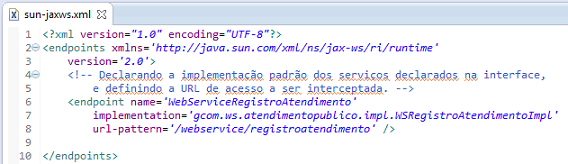
\includegraphics{figuras/declaracao_endpoint.png}
	\caption{Declaração do \textit{EndPoint} dos serviços.}	
	Fonte - Autoria Própria
\end{figure}

Realizado todos esses passos o sistema GSAN conseguirá disponibilizar os novos serviços declarados na interface de Registro de Atendimento, dessa forma o acesso será realizado da seguinte maneira:

\begin{description}
	\item htttp://<servidor>:<porta>/gsan/webservice/registroatendimento
\end{description}

Estando apto a ser integrado com sistemas externos. 